\documentclass{amsart}


\usepackage{fullpage}
\usepackage{graphicx}



\begin{document}
\title{Algoritmi e Strutture Dati\\
Statistica per i big data\\
Esame del 4 Gennaio 2021
}


\newcommand{\NomeStudente}{Giuseppe Persiano}
\newcommand{\nomeClasse}{{\tt{Sol}}}
\newcommand{\nomeMetodo}{{\tt{nuovo}}}
\newcommand{\oraconsegna}{10:35}
\newcommand{\dataoggi}{4 Gennaio, 2021}


\maketitle

\hfill{{\bf Studente: \NomeStudente}}

\smallskip
L'ufficio statistico del comune di Bugliano ha appena scoperto
gli alberi binari e si stanno divertendo non poco con 
la classe {\tt tree} che abbiamo discusso in classe.
Il direttore, che \`e un tipo un po' strano, vi ha chiesto di 
aggiungere alla classe {\tt tree} il metodo {\nomeMetodo} che
sostituisce il valore in ogni nodo con la lista in cui il
primo elemento \`e il minimo dell'albero destro e il secondo elemento
\`e il massimo dell'albero sinistro.
Nel caso in cui un figlio non esista allora si pu\`o assumere che il 
minimo sia $+\infty$ (in {\tt python}, {\tt float('inf')}) e che il massimo
sia $-\infty$ (in {\tt python}, {\tt float('-inf')}).

Ad esempio, l'albero di sinistra dovrebbe essere rimpiazzato con l'albero
che vedete a destra nella figura.

\vskip .8cm

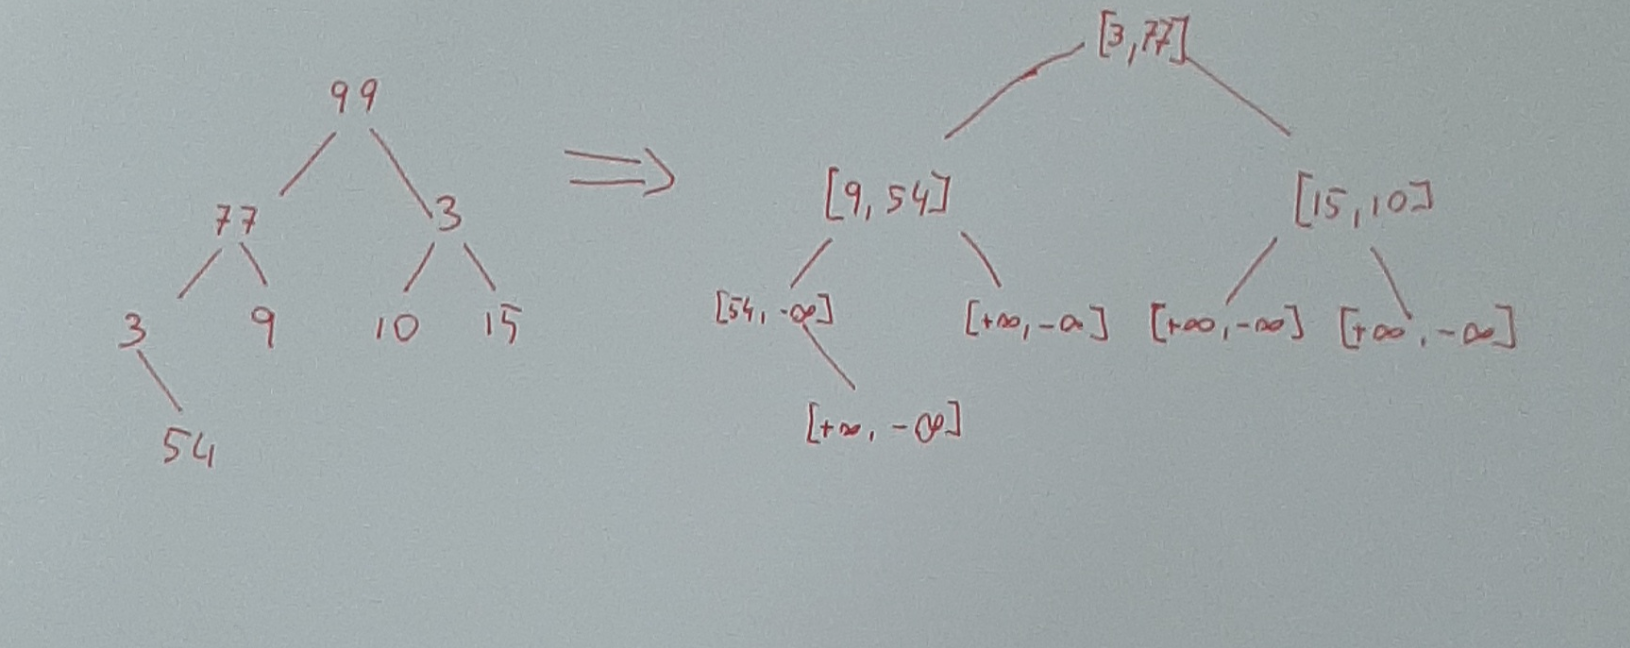
\includegraphics[width=0.8\textwidth]{figura}


\vskip .8cm

\medskip\noindent{\bf Materiale della traccia.}
La cartella contiene il pdf di questa traccia, il file
{\tt alberi.py} che contiene la classe sviluppata in classe,
il file {\tt driver.py} che pu\`o essere usato
per verificare il funzionamento della classe progettata,
e il file  {\tt result.txt} che contiene l'output atteso di {\tt driver.py}.

\medskip\noindent{\bf Istruzione per la consegna.}
Tutto il codice consegnato deve essere aggiunto al file
{\tt alberi.py} ed inviato per e-mail all'indirizzo
{\tt giuper@gmail.com} prima delle ore \oraconsegna\ di oggi, 
\dataoggi. Non inviare altri file e n\'e tantomeno file zip.
Il file consegnato deve poter essere usata per eseguire
il codice di {\tt driver.py}. 


\end{document}
